\begin{figure}[H]
    \centering
    \definecolor{sunorange}{RGB}{238,142,45}
    \definecolor{sunatmos}{RGB}{255,218,145}
    \definecolor{earthblue}{RGB}{76,145,210}
    \definecolor{earthatmos}{RGB}{174,220,245}
    \definecolor{gravityred}{RGB}{185,45,45}
    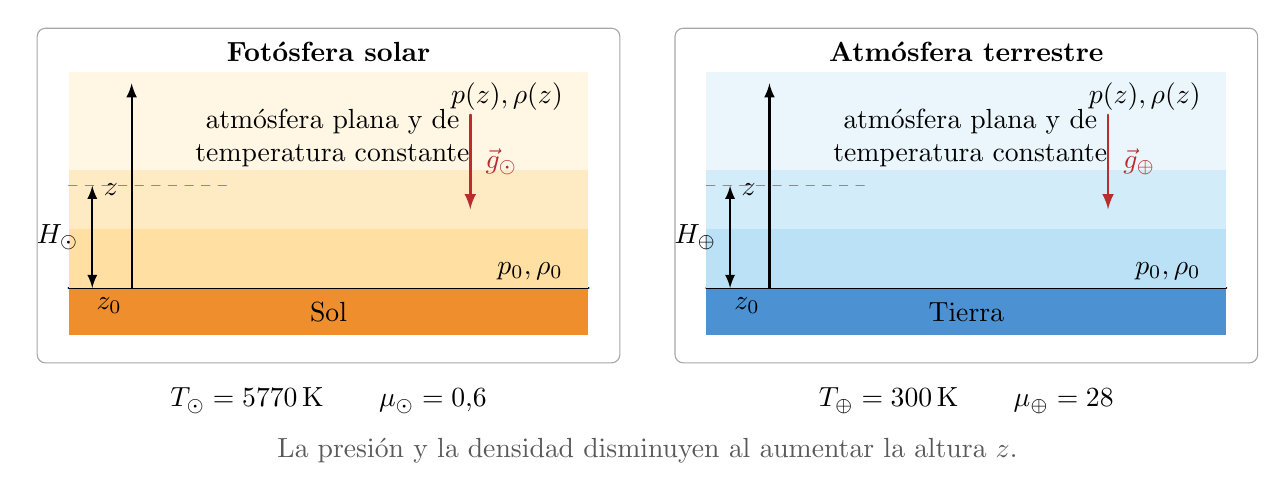
\begin{tikzpicture}[x=1cm,y=1cm,line cap=round,line join=round]
        % Marcos de los dos modelos
        \draw[rounded corners=3pt,black!35]
            (0.25,0.10) rectangle (7.65,4.35);
        \draw[rounded corners=3pt,black!35]
            (8.35,0.10) rectangle (15.75,4.35);

        %----------------------------------------------------------
        % Atmósfera de la fotósfera solar
        \fill[sunorange] (0.65,0.45) rectangle (7.25,1.05);
        \draw[line width=0.95pt] (0.65,1.05) -- (7.25,1.05);
        \fill[sunatmos!85] (0.65,1.05) rectangle (7.25,1.80);
        \fill[sunatmos!55] (0.65,1.80) rectangle (7.25,2.55);
        \fill[sunatmos!25] (0.65,2.55) rectangle (7.25,3.80);

        \node[font=\bfseries] at (3.95,4.05) {Fotósfera solar};
        \node at (3.95,0.75) {Sol};
        \node[align=center] at (4.00,2.95)
            {atmósfera plana y de\\temperatura constante};

        % Coordenada vertical y gravedad
        \draw[-latex,line width=0.75pt] (1.45,1.05) -- (1.45,3.65);
        \node[left] at (1.40,2.30) {$z$};
        \node[below left] at (1.45,1.05) {$z_0$};
        \draw[gravityred,-latex,line width=0.9pt]
            (5.75,3.25) -- (5.75,2.05);
        \node[gravityred,right] at (5.82,2.65) {$\vec g_\odot$};

        % Altura característica y estados termodinámicos
        \draw[dashed,black!45] (0.65,2.35) -- (2.75,2.35);
        \draw[latex-latex,line width=0.65pt] (0.95,1.05) -- (0.95,2.35);
        \node[left] at (0.90,1.70) {$H_\odot$};
        \node[anchor=east] at (7.05,1.27) {$p_0,\rho_0$};
        \node[anchor=east] at (7.05,3.48) {$p(z),\rho(z)$};

        \node[align=center] at (3.95,-0.38)
            {$T_\odot=5770\,\mathrm{K}$\qquad $\mu_\odot=0{,}6$};

        %----------------------------------------------------------
        % Atmósfera terrestre
        \fill[earthblue] (8.75,0.45) rectangle (15.35,1.05);
        \draw[line width=0.95pt] (8.75,1.05) -- (15.35,1.05);
        \fill[earthatmos!85] (8.75,1.05) rectangle (15.35,1.80);
        \fill[earthatmos!55] (8.75,1.80) rectangle (15.35,2.55);
        \fill[earthatmos!25] (8.75,2.55) rectangle (15.35,3.80);

        \node[font=\bfseries] at (12.05,4.05) {Atmósfera terrestre};
        \node at (12.05,0.75) {Tierra};
        \node[align=center] at (12.10,2.95)
            {atmósfera plana y de\\temperatura constante};

        % Coordenada vertical y gravedad
        \draw[-latex,line width=0.75pt] (9.55,1.05) -- (9.55,3.65);
        \node[left] at (9.50,2.30) {$z$};
        \node[below left] at (9.55,1.05) {$z_0$};
        \draw[gravityred,-latex,line width=0.9pt]
            (13.85,3.25) -- (13.85,2.05);
        \node[gravityred,right] at (13.92,2.65) {$\vec g_\oplus$};

        % Altura característica y estados termodinámicos
        \draw[dashed,black!45] (8.75,2.35) -- (10.85,2.35);
        \draw[latex-latex,line width=0.65pt] (9.05,1.05) -- (9.05,2.35);
        \node[left] at (9.00,1.70) {$H_\oplus$};
        \node[anchor=east] at (15.15,1.27) {$p_0,\rho_0$};
        \node[anchor=east] at (15.15,3.48) {$p(z),\rho(z)$};

        \node[align=center] at (12.05,-0.38)
            {$T_\oplus=300\,\mathrm{K}$\qquad $\mu_\oplus=28$};

        % Indicación común del comportamiento con la altura
        \node[black!65,align=center] at (8.00,-1.02)
            {La presión y la densidad disminuyen al aumentar la altura $z$.};
    \end{tikzpicture}
    \caption{Comparación esquemática de las atmósferas planas e isotérmicas consideradas para el Sol y la Tierra. La figura no está a escala.}
\end{figure}
